\newpage
\small\MyriadPro
\label{autora}

\noindent{}COLABORADORES\\

\noindent{}AURORA FORNONI BERNARDINI


\begin{wrapfigure}{l}{4cm}
%\begin{minipage}{0,4\textwidth}
%\centering
  \includegraphics[width=35mm]{./imgs/aurora.jpg}
%\caption{I}
%\end{minipage}
 \end{wrapfigure}


É professora, escritora e tradutora. Nasceu em
8 de julho de 1941 em Domodossola, Novara (Itália), e em 1954 veio com a
família para o Brasil. Graduou"-se em inglês (1959--1963) e em russo
(1962--1966) pela Universidade de São Paulo, onde ainda concluiu seu
mestrado (1970, sob orientação de Boris Schnaiderman) e doutorado (1973,
sob orientação de Alfredo Bosi) sobre o futurismo russo e italiano, e
sua livre"-docência (1978) sobre Marina Tsvetáieva. Morou períodos na
França, na Inglaterra e na Rússia, aperfeiçoando os idiomas.

Começou a estudar russo em 1958 e, no fim da década de 1960, durante o
mestrado, foi convidada para lecionar na \scalebox{0.8}{USP} por Boris Schnaiderman
(1917--2016), o primeiro professor do curso de língua e de literatura
russa da universidade. Atualmente Aurora Bernardini é professora titular
de pós"-graduação nos programas de Literatura e Cultura Russa (atual
\scalebox{0.8}{LETRA}) e de Teoria Literária e Literatura Comparada (\scalebox{0.8}{FFLCH/USP}), tendo
orientado dezenas de alunos.

Começou a trabalhar como tradutora em 1969, na ocasião da preparação de
seu mestrado sobre o futurismo. Já traduziu mais de cinquenta livros,
muitos deles do idioma russo. Como escritora, com o pseudônimo de Vera
Albers, publicou livros como \emph{Deformação} (Ed. Perspectiva, 1980) e
\emph{Surtos urbanos} (ed. 34, 1998). É organizadora de muitos volumes,
como \emph{O futurismo italiano: manifestos} (Ed. Perspectiva, 1980),
\emph{Mitopoéticas: da Rússia às Américas} (Associação Editorial
Humanitas, 2006, com Jerusa Pires Ferreira), e \emph{A estrutura do
conto de magia} (\scalebox{0.8}{UFSC}, 2015, com S. I. Nekliúdov). Colaboradora assídua
de vários periódicos, como dos jornais \emph{Folha de S. Paulo} e
\emph{Estado de S. Paulo} e da revista \scalebox{0.8}{\emph{CULT}}. Também ministra
cursos e palestras sobre literatura e tradução, na Casa das Rosas, Casa
Guilherme de Almeida, Centro Universitário Maria Antonia (\scalebox{0.8}{USP}), etc.

Aurora Fornoni Bernardini ainda se dedica à pintura, tendo realizado
exposições individuais e coletivas.

Algumas traduções do russo: \emph{Ka}, de Velimir Khlébnikov
(Perspectiva, 1977); \emph{Réquiem}, de Anna Akhmátova (com Hadasa
Cytrynowicz, Art Editora, 1991); \emph{Os arquétipos literários}, de
Eleazar Meletínski (cotradução, Ed. Ateliê Editorial, 1998); \emph{O
Tenente Quetange}, de Iúri Tyniánov (CosacNaify, 2002); \emph{Cartas a
Suvórin (1886--1891),} de Anton Tchékhov (com Homero Freitas de Andrade,
Ed. Edusp, 2002); \emph{Maria: uma peça e cinco histórias}, de Isaac
Bábel (com Homero Freitas de Andrade, CosacNaify, 2003);
\emph{Enfermaria nº 6,} de Anton Tchékhov (Ed. Veredas, 2005);
\emph{Indícios flutuantes}, antologia de poemas de Marina Tsvetáieva
(Martins Fontes, 2006); \emph{O exército de cavalaria}, de Isaac Bábel
(com Homero Freitas de Andrade, CosacNaify, 2006); \emph{Vivendo sob o
fogo: confissões}, de Marina Tsvetáieva (Ed. Martins, 2008); \emph{Dos
diários de Serguei Eisenstein e outros ensaios}, de Viatchesláv Ivánov
(com Noé Silva, Ed. Edusp, 2009); \emph{Nova antologia do conto russo
(1792--1998)} com as traduções dos contos ``Taman'', de Mikhail
Lêrmontov, e ``Liompa'', de Iúri Oliecha (Ed. 34, 2011); ``\emph{Os
sonhos teus vão acabar contigo'': prosa, poesia, teatro}, de Daniil
Kharms (com Daniela e Moissei Mountian, Ed. Kalinka, 2013); \emph{Poesia
russa: seleta bilíngue}, com poemas de Aleksándr Púchkin, Mikhail
Lêrmontov, Aleksándr Blok, Anna Akhmátova, Boris Pasternak, etc. (Ed.
Kalinka, 2016); \emph{Luminescência: antologia poética}, de Viatchesláv
Kupriyánov (Ed. Kalinka, 2016); \emph{Tarakã: o bigodudo}, de Kornei
Tchukóvski (com Maria Vragova, Ed. Kalinka e Ars et Vita, 2016).

Premiações: em 2003, foi finalista do Jabuti pela cotradução de
\emph{Cartas a Suvórin}, de Anton Tchékhov (Edusp); em 2004, recebeu o
prêmio Jabuti (segundo lugar), com o poeta Haroldo de Campos, pela
tradução de \emph{Ungaretti: daquela estrela à outra} (Ed. Ateliê
Editorial); em 2006, foi vencedora do prêmio \scalebox{0.8}{APCA} pela cotradução de
\emph{O exército de cavalaria}, de Isaac Bábel (CosacNaify); em 2006,
foi contemplada com o prêmio Paulo Rónai pela tradução de \emph{Indícios
flutuantes -- poemas}, de Marina Tsvetáieva (Martins Fontes); em 2007, foi
vencedora do prêmio Jabuti (terceiro lugar) também pela tradução de
\emph{Indícios flutuantes}; em 2014, foi finalista do Jabuti pela
cotradução de \emph{``Os sonhos teus vão acabar contigo'': prosa,
poesia, teatro}, de Daniil Kharms (Kalinka).

\medskip

\noindent{}ARLETE CAVALIERE é ensaísta, tradutora e professora titular de Teatro,
Arte e Cultura Russa no curso de graduação e pós"-graduação do
Departamento de Letras Orientais (\scalebox{0.8}{FFLCH}) da Universidade de São Paulo. É
mestre e doutora em Teoria Literária e Literatura Comparada e
livre-docente pela \scalebox{0.8}{USP}, com pesquisas sobre a prosa e o teatro de Gógol
e a estética teatral do vanguardista Meyerhold. Entre 2002 e 2004 atuou
como professora"-leitora do Brasil na Universidade Estatal de Moscou
Lomonóssov (\scalebox{0.8}{MGU}). Organizou com colegas docentes da \scalebox{0.8}{USP} publicações
coletivas, como a revista \emph{Caderno de Literatura e Cultura
Russa} (Ateliê Editorial, 2004 e 2008) e os livros \emph{Tipologia do
simbolismo nas culturas russa e ocidental} (Humanistas, 2005) e
\emph{Teatro russo: literatura e espetáculo} (Ateliê Editorial, 2011). É
autora de \emph{Teatro russo: percurso para um estudo da paródia
e do grotesco} (Humanistas, 2009). Também publicou diversas traduções,
entre elas: \emph{O nariz \& A terrível vingança}, de Nikolai
Gógol (Edusp, 1990), com o ensaio ``A magia das máscaras''; \emph{O
inspetor geral de Gógol/Meyerhold: um espetáculo síntese} (Perspectiva,
1996), com ensaio crítico sobre a poética de Meyerhold; \emph{Ivánov},
de Anton Tchékhov (Edusp, 1998, cotradutora, finalista Jabuti de
tradução); \emph{Teatro completo}, de Nikolai Gógol (Editora 34, 2009,
também organizadora); \emph{Mistério"-bufo}, de Vladímir Maiakóvski (Ed.
34, 2012, com ensaio); e \emph{Dostoiévski"-trip}, de Vladímir Sorókin
(Ed. 34, 2014, com ensaio). Escreveu o texto de apresentação de
\emph{Clássicos do conto russo} (Ed. 34, 2015) e participou da
\emph{Nova antologia do conto russo (1792--1998)} (Ed. 34, 2011, org.
Bruno Barreto Gomide). É ainda organizadora e prefaciadora da
\emph{Antologia do humor russo (1823--2014)} (Editora 34, 2018).


\medskip

\noindent{}DANIELA MOUNTIAN é tradutora, designer e editora da \emph{Kalinka},
dedicada à cultura russa. Fez pela \scalebox{0.8}{USP} graduação em história, mestrado
sobre Fiódor Sologub e doutorado"-sanduíche sobre Daniil Kharms, com
estágio de um ano na Casa de Púchkin, em São Petersburgo. Atualmente,
desenvolve pós"-doutorado sobre literatura infantil russa e brasileira no
programa de Teoria Literária e Literatura Comparada (\scalebox{0.8}{USP}). Traduziu com
seu pai, Moissei Mountian, o conto ``Luz e sombras'', de Fiódor Sologub,
para a \emph{Nova antologia do conto russo} (Editora 34, 2011); a
coletânea \emph{Os sonhos teus vão acabar contigo}, de Daniil Kharms
(Kalinka, 2013, também com Aurora Bernardini); e os volumes \emph{Diário
de um escritor (1873): Meia carta de um sujeito}, de Fiódor Dostoiévski
(Hedra, 2016), e \emph{A ressurreição do lariço} (\emph{Contos de Kolimá
5}), de Varlam Chalámov (Ed. 34, 2016). Com Yulia Mikaelyan, Daniela
verteu \emph{O ofício}, de Serguei Dovlátov (Kalinka, 2017).

\medskip

\noindent{}VALTEIR VAZ é formado em Letras pelo Centro Universitário Fundação Santo
André, mestre em Teoria Literária e Literatura Comparada (\scalebox{0.8}{USP}) e doutor
em Literatura e Cultura Russa (\scalebox{0.8}{USP}). É professor na área de Língua
Portuguesa, Literatura, Redação e Metodologia Científica no Centro
Estadual de Educação Tecnológica Paula Souza (\scalebox{0.8}{ETEC} e \scalebox{0.8}{FATEC}). É professor
colaborador do programa de pós"-graduação em Literatura e Cultura Russa
(\scalebox{0.8}{LETRA/USP}).

\medskip

\noindent{}PAULO HENRIQUE POMPERMAIER é graduado em Jornalismo pela Faculdade Cásper Líbero e graduando em Letras pela \scalebox{0.8}{USP}. Como repórter atuou na Revista \scalebox{0.8}{\emph{CULT}} e atualmente é editor-assistente da Hedra.

\afterpage{\blankpage}

\newpage
\pagestyle{empty}
\MyriadPro

\noindent{}Catálogo da editora Kalinka\\[5pt]

\noindent{}O Diabo Mesquinho\\
FIÓDOR SOLOGUB
\medskip

\noindent{}Encontros com Liz e outras histórias\\
LEONID DOBÝTCHIN
\medskip

\noindent{}``Os sonhos teus vão acabar contigo'': prosa, poesia, teatro\\
DANIIL KHARMS
\medskip

\noindent{}Luminescência: antologia poética\\
VIATCHESLÁV KUPRIYÁNOV
\medskip

\noindent{}Luminescência: desdobramentos\\
VIATCHESLÁV KUPRIYÁNOV
\medskip

\noindent{}Poesia russa: seleta bilíngue
\medskip

\noindent{}Tarakã, o bigodudo (Ars et Vita e Kalinka)\\
KORNEI TCHUKÓVSKI
\medskip

\noindent{}Parque Cultural\\
SERGUEI DOVLÁTOV
\medskip

\noindent{}Salmo\\
FRIEDRICH GORENSTEIN
\medskip

\noindent{}O ofício\\
SERGUEI DOVLÁTOV
\medskip

\noindent{}O elefante (Coleção Mir)\\
ALEKSANDR KUPRIN
\medskip

\noindent{}A velha (Coleção Mir)\\
DANIIL KHARMS 
\medskip

\noindent{}Bobók \& `Meia carta' de sujeito (Coleção Mir)\\
FIÓDOR DOSTOIÉVSKI
\medskip

\noindent{}Aulas de literatura russa: de Púchkin a Gorenstein \\
AURORA FORNONI BERNARDINI

\newpage
\pagestyle{empty}
\MyriadPro
\scriptsize
\begin{center}
AULAS DE LITERATURA RUSSA\\[6pt]

Copyright © 2018, Editora Kalinka\\[6pt]

All rights reserved\\[20pt]

Organização © Daniela Mountian e Valteir Vaz, 2018\\[6pt]

Prefácio © Arlete Cavaliere, 2018\\[6pt]

primeira edição, 2018\\[40pt]


Essa publicação está de acordo com a reforma ortográfica.\\[6pt]
A imagem da capa foi baseada num tecido de Leon Bakst (1866--1924).\\[6pt]	
Agradecimentos: Arlete Cavaliere, Belkiss Rabello, Irineu Franco Perpetuo, João Luiz Sampaio, Jorge Sallum, Maria Fernanda Rodrigues, Paulo Henrique Pompermaier, Suzana Salama e Valteir Vaz; Ateliê Editorial, \scalebox{0.8}{CULT}, Estado de S. Paulo, Editora Perspectiva, Editora \scalebox{0.8}{UFPE}, Folha de S. Paulo, Martins Editora, Revista Acta Semiótica et Lingvistica, Revista Ciência Hoje, Revista da Biblioteca Mário de Andrade, Revista Literatura e Sociedade, Revista Outra travessia, Revista Qorpus, Revista \scalebox{0.8}{RUS}, Revista Tradterm, Revista \scalebox{0.8}{USP}, Theatro Municipal.\\[20pt]
\end{center}


\bigskip

\begin{vplace}[1]
\begin{table}[ht!]
\MyriadPro
\scriptsize
\begin{tabular}{rl}
TÍTULO            & Aulas de literatura russa: de Púchkin a Gorenstein \\[2pt]
AUTOR             & Aurora Fornoni Bernardini                          \\[2pt]
PREFÁCIO          & Arlete Cavaliere                                   \\[2pt]
ORGANIZAÇÂO       & Daniela Mountian e Valteir Vaz                     \\[2pt]
REVISÃO           & Daniela Mountian e Paulo Henrique Pompermaier      \\[2pt]
EDIÇÃO            & Kalinka                                            \\[2pt]
PRODUÇÃO EXECUTIVA & Hedra                                             \\[2pt]
EDITORA           & Daniela Mountian                                   \\[2pt] 
EDITOR-ASSISTENTE & Paulo Henrique Pompermaier                         \\[2pt]
CAPA              & Daniela Mountian                                   \\[2pt]
PROJETO GRÁFICO   & Kalinka                                            \\[2pt]
FORMATO           & 14 x 21 cm                                         \\[2pt]
NÚMERO de PÁGINAS & 436                                                \\[2pt]
ISBN              & 978-85-61096-18-2                                 
\end{tabular}
\end{table}
\end{vplace}

\newpage
\MyriadPro
\begin{center}
\small
Aulas de literatura russa
\end{center}

\scriptsize


\begin{figure}[!ht]
%\begin{minipage}{2\textwidth}
\centering

  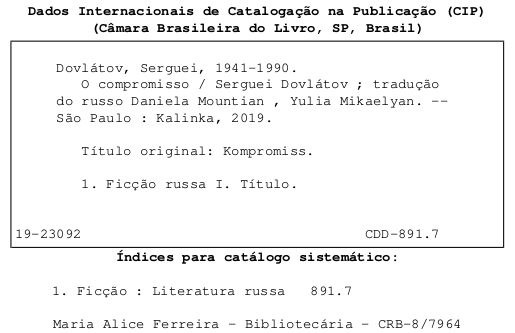
\includegraphics[width=80mm]{./imgs/ficha.jpg}
%\caption{I}
%\end{minipage}
 \end{figure}


%\begin{vplace}[1]
%\begin{center}
%Dados Internacionais de Catalogação na Publicação (CIP)\\
%(Câmara Brasileira do Livro, SP, Brasil)\\
%\_\_\_\_\_\_\_\_\_\_\_\_\_\_\_\_\_\_\_\_\_\_\_\_\_\_\_\_\_\_\_\_\_\_\_\_\_\_\_\_\_\_\_\_\_\_\_\_\_\_\_\_\_\_\_\_\_\_\_\\
%\end{center}
%\hspace{30pt}Bernardini, Aurora Fornoni, XXXX--


%\hspace{35pt}Aulas de literatura russa : de Púchkin a Gorenstein / Aurora Fornoni

%\hspace{12pt}Bernardini ; organização Valteir Vaz ; prefácio Arlete Cavaliere. - - São Paulo :

%\hspace{12pt}Kalinka, 2018.\\[6pt]

%\hspace{35pt}ISBN XXX-XX-XXXXX-XX-X\\[6pt]

%\hspace{35pt}1. Literatura russa II. Crítica literária III. Título.

%\begin{center}
%\hspace{10pt}XX-XXXXX \hspace{180pt}CDD-XXX.X
%\_\_\_\_\_\_\_\_\_\_\_\_\_\_\_\_\_\_\_\_\_\_\_\_\_\_\_\_\_\_\_\_\_\_\_\_\_\_\_\_\_\_\_\_\_\_\_\_\_\_\_\_\_\_\_\_\_\_\_\\
%Índices para catálogo sistemático:\\[3pt]
%1. Crítica literária : Literatura russa XXX.X\\
%\end{center}
%\end{vplace}

\begin{center}
EDIÇÃO: EDITORA KALINKA\\[7pt]
Rua Imaculada Conceição, 41 cj. 03\\[7pt]
01226-020 São Paulo-SP Tel.11 2579-6290\\[7pt]
www.kalinka.com.br\\[30pt]

PRODUÇÃO EXECUTIVA: EDITORA HEDRA\\[7pt]
Rua Fradique Coutinho, 1139 Vila Madalena\\[7pt]
05416-011 São Paulo-SP Tel.11 3097-8304\\[7pt]
www.hedra.com.br
\end{center}

%TÍTULO Aulas de literatura russa: de Púchkin a Gorenstein\\
%AUTOR Aurora Fornoni Bernardini\\
%REVISÃO Daniela Mountian e Paulo Henrique Pompermaier\\
%EDIÇÃO Hedra\\
%CAPA Daniela Mountian\\
%PROJETO GRÁFICO Hedra\\
%FORMATO 14 x 21 cm\\
%NÚMERO de PÁGINAS 398\\
%ISBN XXX-XX-XXXXX-XX-X\\